\section{Datenbank}
\label{sec:Entwurf-Datenbank}
Im Gegensatz zur bestehenden Anwendung wird auf eine relationale Datenbank anstatt auf Dateien zurückgegriffen. Das Vorgehen resultiert unter anderem aus der gestiegenen Datenmenge. Eine NoSQL-Datenbank wird nicht benötigt, da sich alle Daten in Schemen untergliedern lassen und häufige Änderungen vorgesehen sind. Die Nutzung einer Datenbank stellt sicher, dass sich die Daten an einer zentralen Stelle befinden und nicht über die Anwendung verstreut sind. Auch wird eine mögliche Redundanz von Daten verhindert, da in Datenbanken mit Relationen gearbeitet werden kann. Durch die AKID-Eigenschaft (Atomarität, Konsistenz, Isolation und Dauerhaftigkeit) der Datenbanken wird sichergestellt, dass Daten in der Datenbank vollständig und konsistent sind. Ferner sind die Abfragen an eine Datenbank besser optimiert, als Abfragen auf eine Datei. \cite{drillingWasIstDatenbank2017}

Es ist möglich, die Punkteberechnung in der Datenbank unter Zuhilfenahme von \textit{Views} durchzuführen.

\subsection{Basis-Tabellen}
\begin{center}
	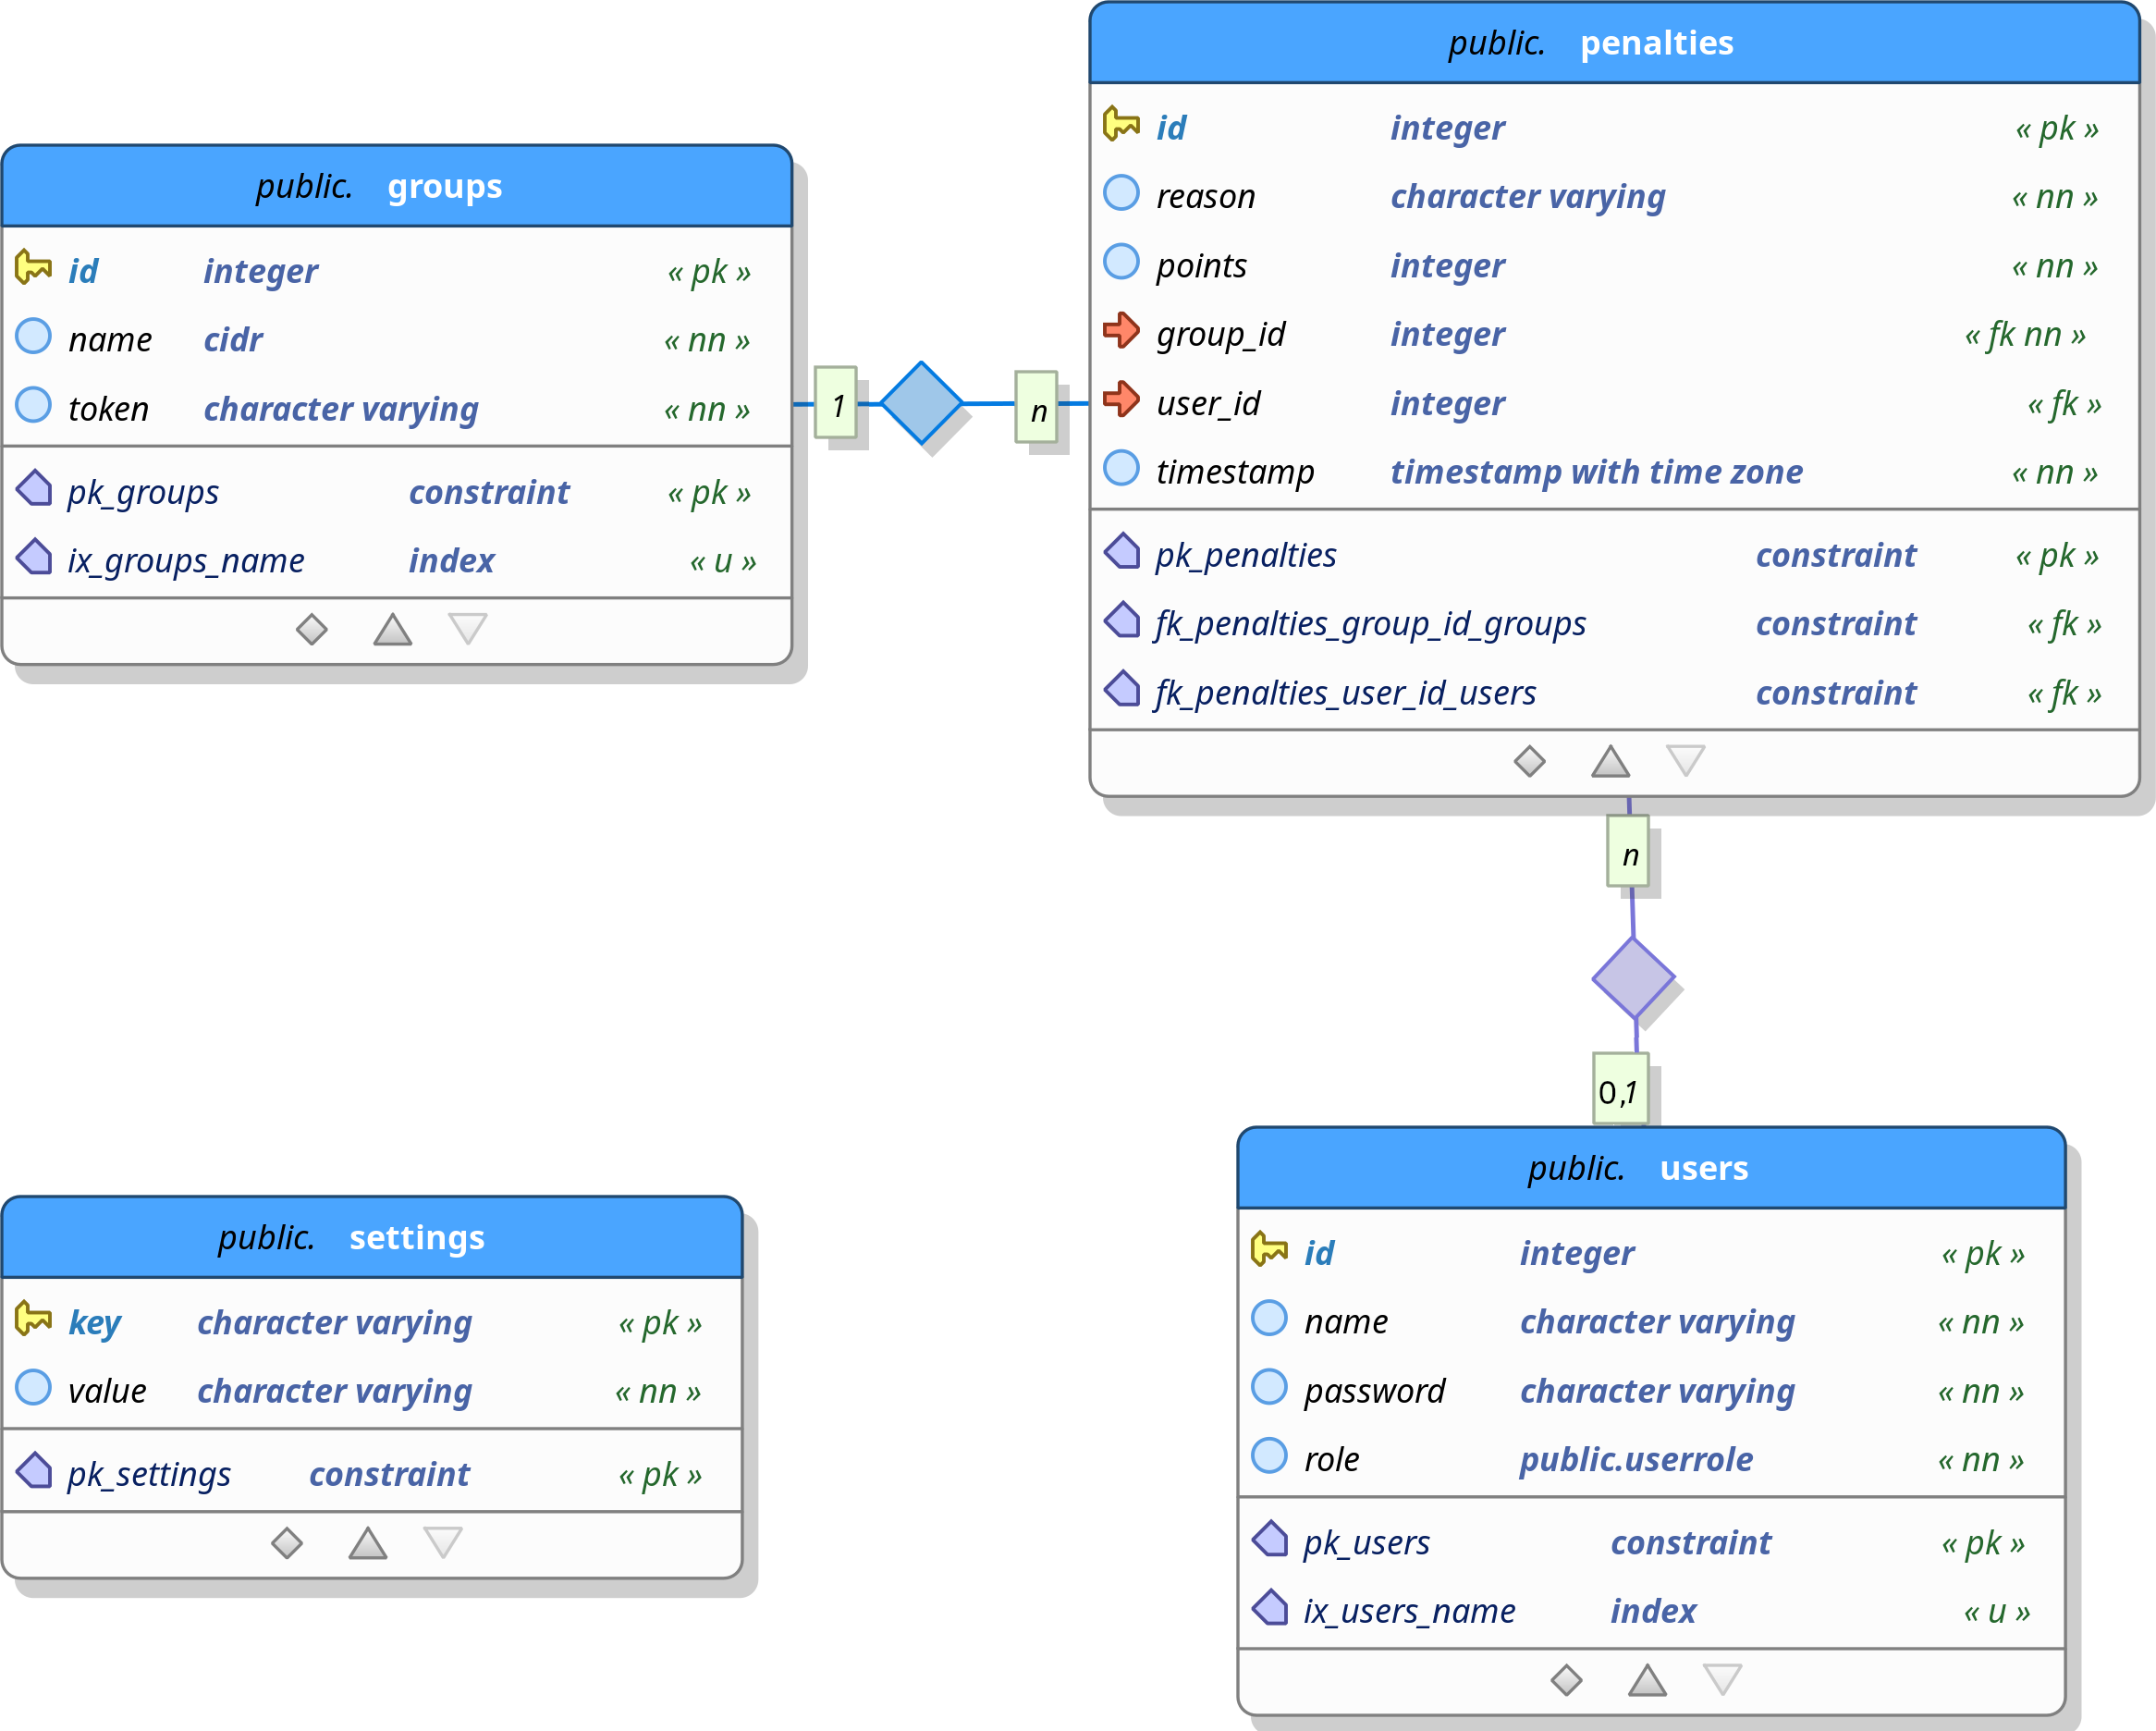
\includegraphics[width=\linewidth, keepaspectratio]{entwurf/datenbank/basis-tabellen}
	\captionof{figure}{Ansicht der Basis-Tabellen (ER-Diagramm)}
	\label{fig:db-basis-table}
\end{center}

In der \autoref{fig:db-basis-table} ist neben der alleinstehenden Tabelle \textbf{\textit{settings}} die Tabelle \textbf{\textit{users}} sowie die n:m-Beziehung  zwischen \textbf{\textit{users}} und \textbf{\textit{groups}} dargestellt. Die  n:m-Beziehung wird über eine Referenztabelle (\textbf{\textit{penalties}}) mit einer 1:n-Beziehung zwischen \textbf{\textit{groups}} und \textbf{\textit{penalties}} und einer 0,1:n-Beziehung zwischen \textbf{\textit{users}} und \textbf{\textit{penalties}} modelliert. In der n:m-Beziehung werden die ausgesprochenen Strafen gespeichert. Jede Gruppe kann von mehreren betreuenden Personen oder dem System mehrmals verwarnt werden.

\subsubsection{Einstellungen}
Die \textbf{\textit{settings}}-Tabelle beinhaltet Einstellungen des Spiels als key-value Paar. Hierbei sind beide Spalten Strings und Key einzigartig. Zu den Einstellungen gehören beispielsweise das Scan-Intervall, die Anzahl der Flags pro Team sowie das Ende der Discover- und Attackzeit.

\subsubsection{Account}
In der Tabelle \textbf{\textit{users}} sind die Login-Informationen der administrierenden, der betreuenden und der spielenden Personen hinterlegt. Da der Login aus Nutzername und Passwort besteht, werden die Spalten \textit{name} und \textit{password} benötigt. Auch muss anhand des Nutzernamens eindeutig auf einen Account geschlossen werden, deshalb ist die Spalte \textit{name} als unique gekennzeichnet. Die Rolle des Accounts wird mithilfe eines Enums (\textit{role}) definiert. Ein Enum ist eine Liste von benannten Werten.

\subsubsection{Strafen}
Die durch das System oder die betreuenden Personen verteilten Strafen werden in der Tabelle \textbf{\textit{penalties}} gespeichert. Dazu wird neben dem Grund der Strafe (\textit{reason}), dem Zeitpunkt der Bestrafung (\textit{timestamp}), auch die Anzahl an Strafpunkten (\textit{points}) festgehalten. Damit Gruppen von einer betreuenden Person öfters bestraft werden können, ist der Primärschlüssel des Eintrages die ID der Strafe.

\subsection{Gruppen-Tabellen}
\begin{center}
	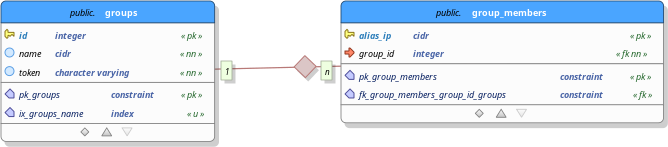
\includegraphics[width=\linewidth, keepaspectratio]{entwurf/datenbank/gruppen-tabellen}
	\captionof{figure}{Ansicht der Gruppen-Tabellen (ER-Diagramm)}
	\label{fig:db-group-table}
\end{center}

Wie in \autoref{fig:db-group-table} zu sehen ist, existiert zwischen der Tabelle \textbf{\textit{groups}} und \textbf{\textit{group\_members}} eine 1:n-Beziehung. Dies bedeutet, dass eine Gruppe mehrere Mitglieder haben kann, aber jedes Mitglied nur genau in einer Gruppe vertreten sein kann.

\subsubsection{Gruppe}
In der Tabelle \textbf{\textit{groups}} werden alle teilnehmenden GameClients vermerkt. Jede Gruppe besitzt eine eindeutige \textit{ID} und einen eindeutigen \textit{Namen}. Der \textit{Name} der Gruppe repräsentiert die IP-Adresse des GameClients und ist nach der \textit{Classless Internet Domain Routing (CIDR)} Konvention abgelegt. Des Weiteren besitzt die \textbf{\textit{groups}} Tabelle die Spalte \textit{token}. In dieser wird der individuelle Token, der zur Flaggenerierung benötigt wird, abgespeichert. Dies ist nötig, damit der Server dieselben Flags wie der GameClient generieren kann und die betreuenden Personen die Korrektheit verifizieren können.

\subsubsection{Gruppenmitglieder}
Die Tabelle \textbf{\textit{group\_members}} beinhaltet alle IP-Adressen, die im Namen einer Gruppe agieren dürfen. Dafür wird die IP-Adresse im Feld \textit{alias\_ip} und die vertretende Gruppe als Referenz im Feld \textit{group\_id} gespeichert. Da das Feld \textit{alias\_ip} als Primärschlüssel verwendet wird, kann jede IP-Adresse nur genau eine Gruppe vertreten.

\subsection{Flags-Tabellen}
\begin{center}
	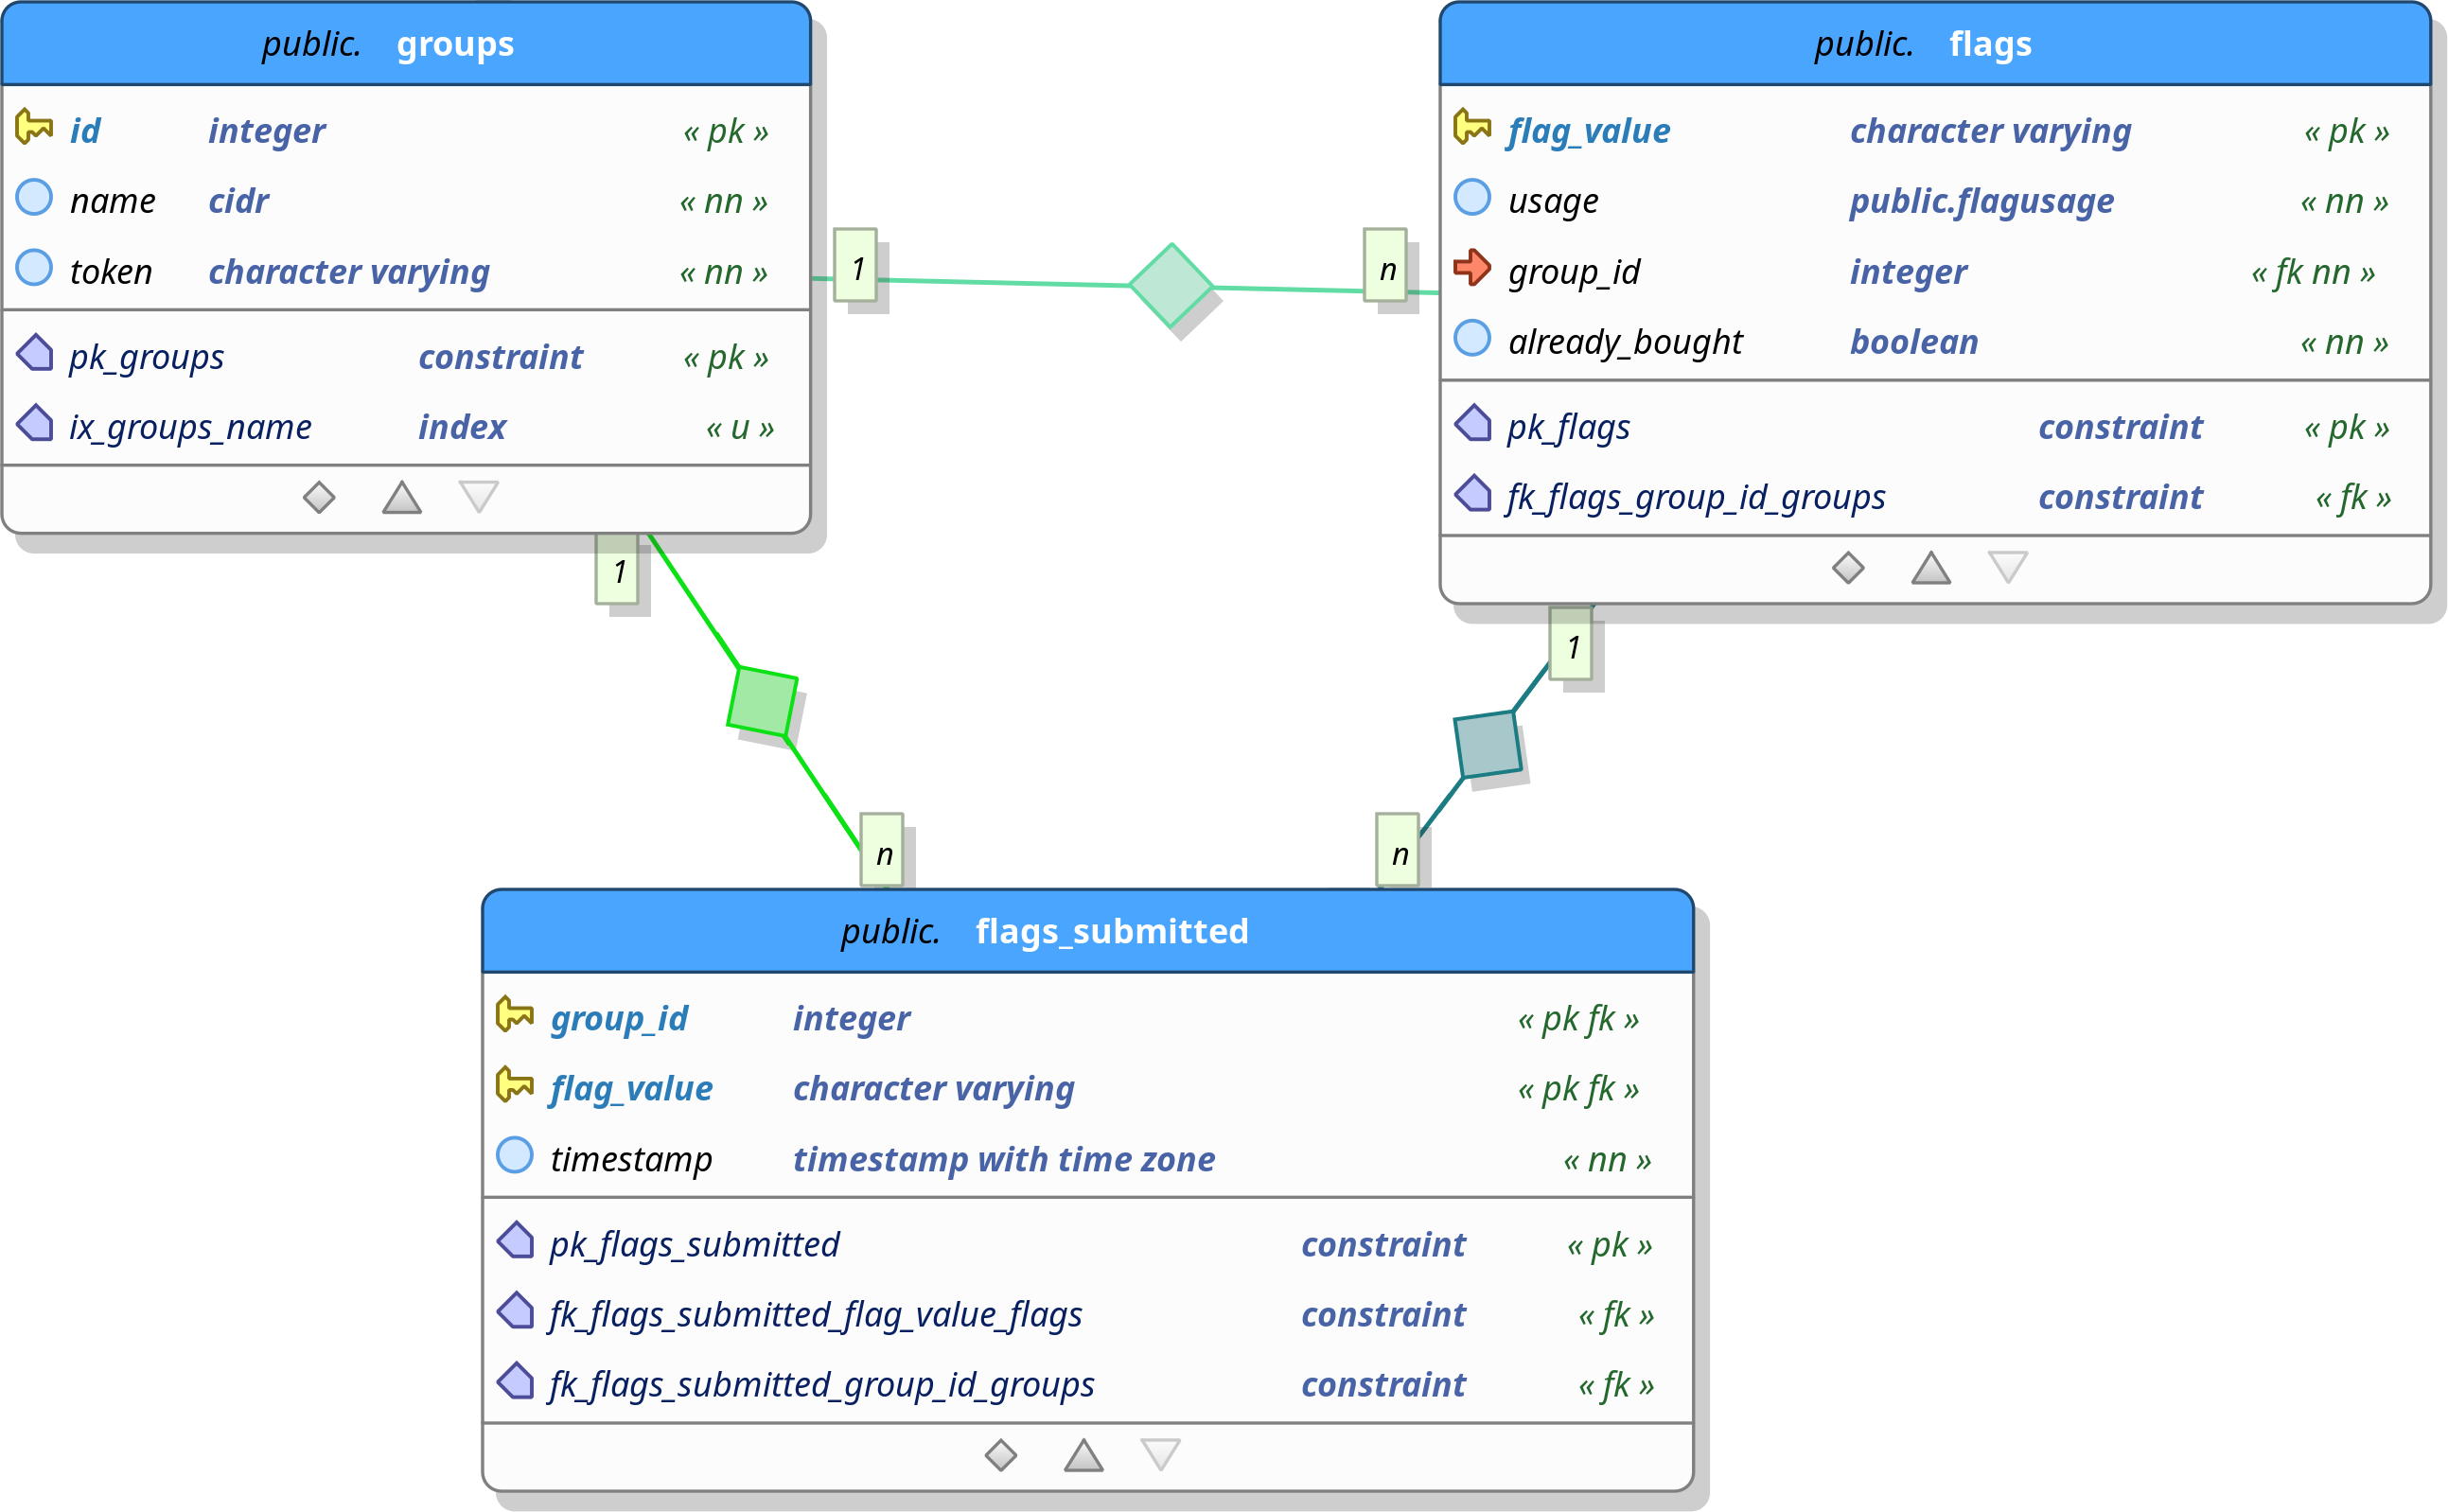
\includegraphics[width=\linewidth, keepaspectratio]{entwurf/datenbank/flags-tabellen}
	\captionof{figure}{Ansicht der Flags-Tabellen (ER-Diagramm)}
	\label{fig:db-flags-table}
\end{center}


In der \autoref{fig:db-flags-table} ist die 1:n-Beziehung zwischen den Tabellen \textbf{\textit{groups}} und \textbf{\textit{flags}} erkennbar. Dieses hat zur Folge, dass eine Gruppe mehrere Flags besitzen kann, jedoch eine Flag immer genau zu einer Gruppe gehört. In der Abbildung ist weiter die n:m-Beziehung zwischen \textbf{\textit{groups}} und \textbf{\textit{flags}} abgebildet. Diese wird in eine Verknüpfungstabelle namens \textbf{\textit{flags\_submitted}} mit zwei 1:n-Beziehung zerlegt. Diese Tabelle enthält die abgegebenen Flags.
 
\subsubsection{Flags}
Die während eines Spiels generierten und benötigten Flags werden in der Tabelle \textbf{\textit{flags}} abgelegt. Hierzu wird der Wert einer Flag als String in der Spalte \textit{flag\_value} festgehalten. Auch wird die Nutzungsart unter Zuhilfenahme eines Enums und die Gruppenzugehörigkeit als Referenz gespeichert. Außerdem wird in der Spalte \textit{already\_bought} als Bool vermerkt, ob diese Flag bereits im Flagshop erworben wurde. Diese Spalte besitzt nur Relevanz für die dementsprechenden Flagshop Flags und wird bei den übrigen Flags ignoriert.

\subsubsection{Abgegebene Flags}
Die durch die Studierenden abgegebenen Flags werden in der Tabelle \textbf{\textit{flags\_submitted}} eingetragen. Auch wird der Zeitpunkt der Abgabe mitgespeichert, um eventuelle Betrugsversuche aufzudecken. Die Spalten \textit{group\_id} und \textit{flag\_value} bilden zusammen den Primärschlüssel. Dieses ermöglicht, dass jede Gruppe jede Flag abgeben kann. Die Mehrfachabgabe einer Flag durch eine Gruppe wird so auch unterbunden.

\clearpage
\subsection{Service-Tabellen}
\begin{center}
	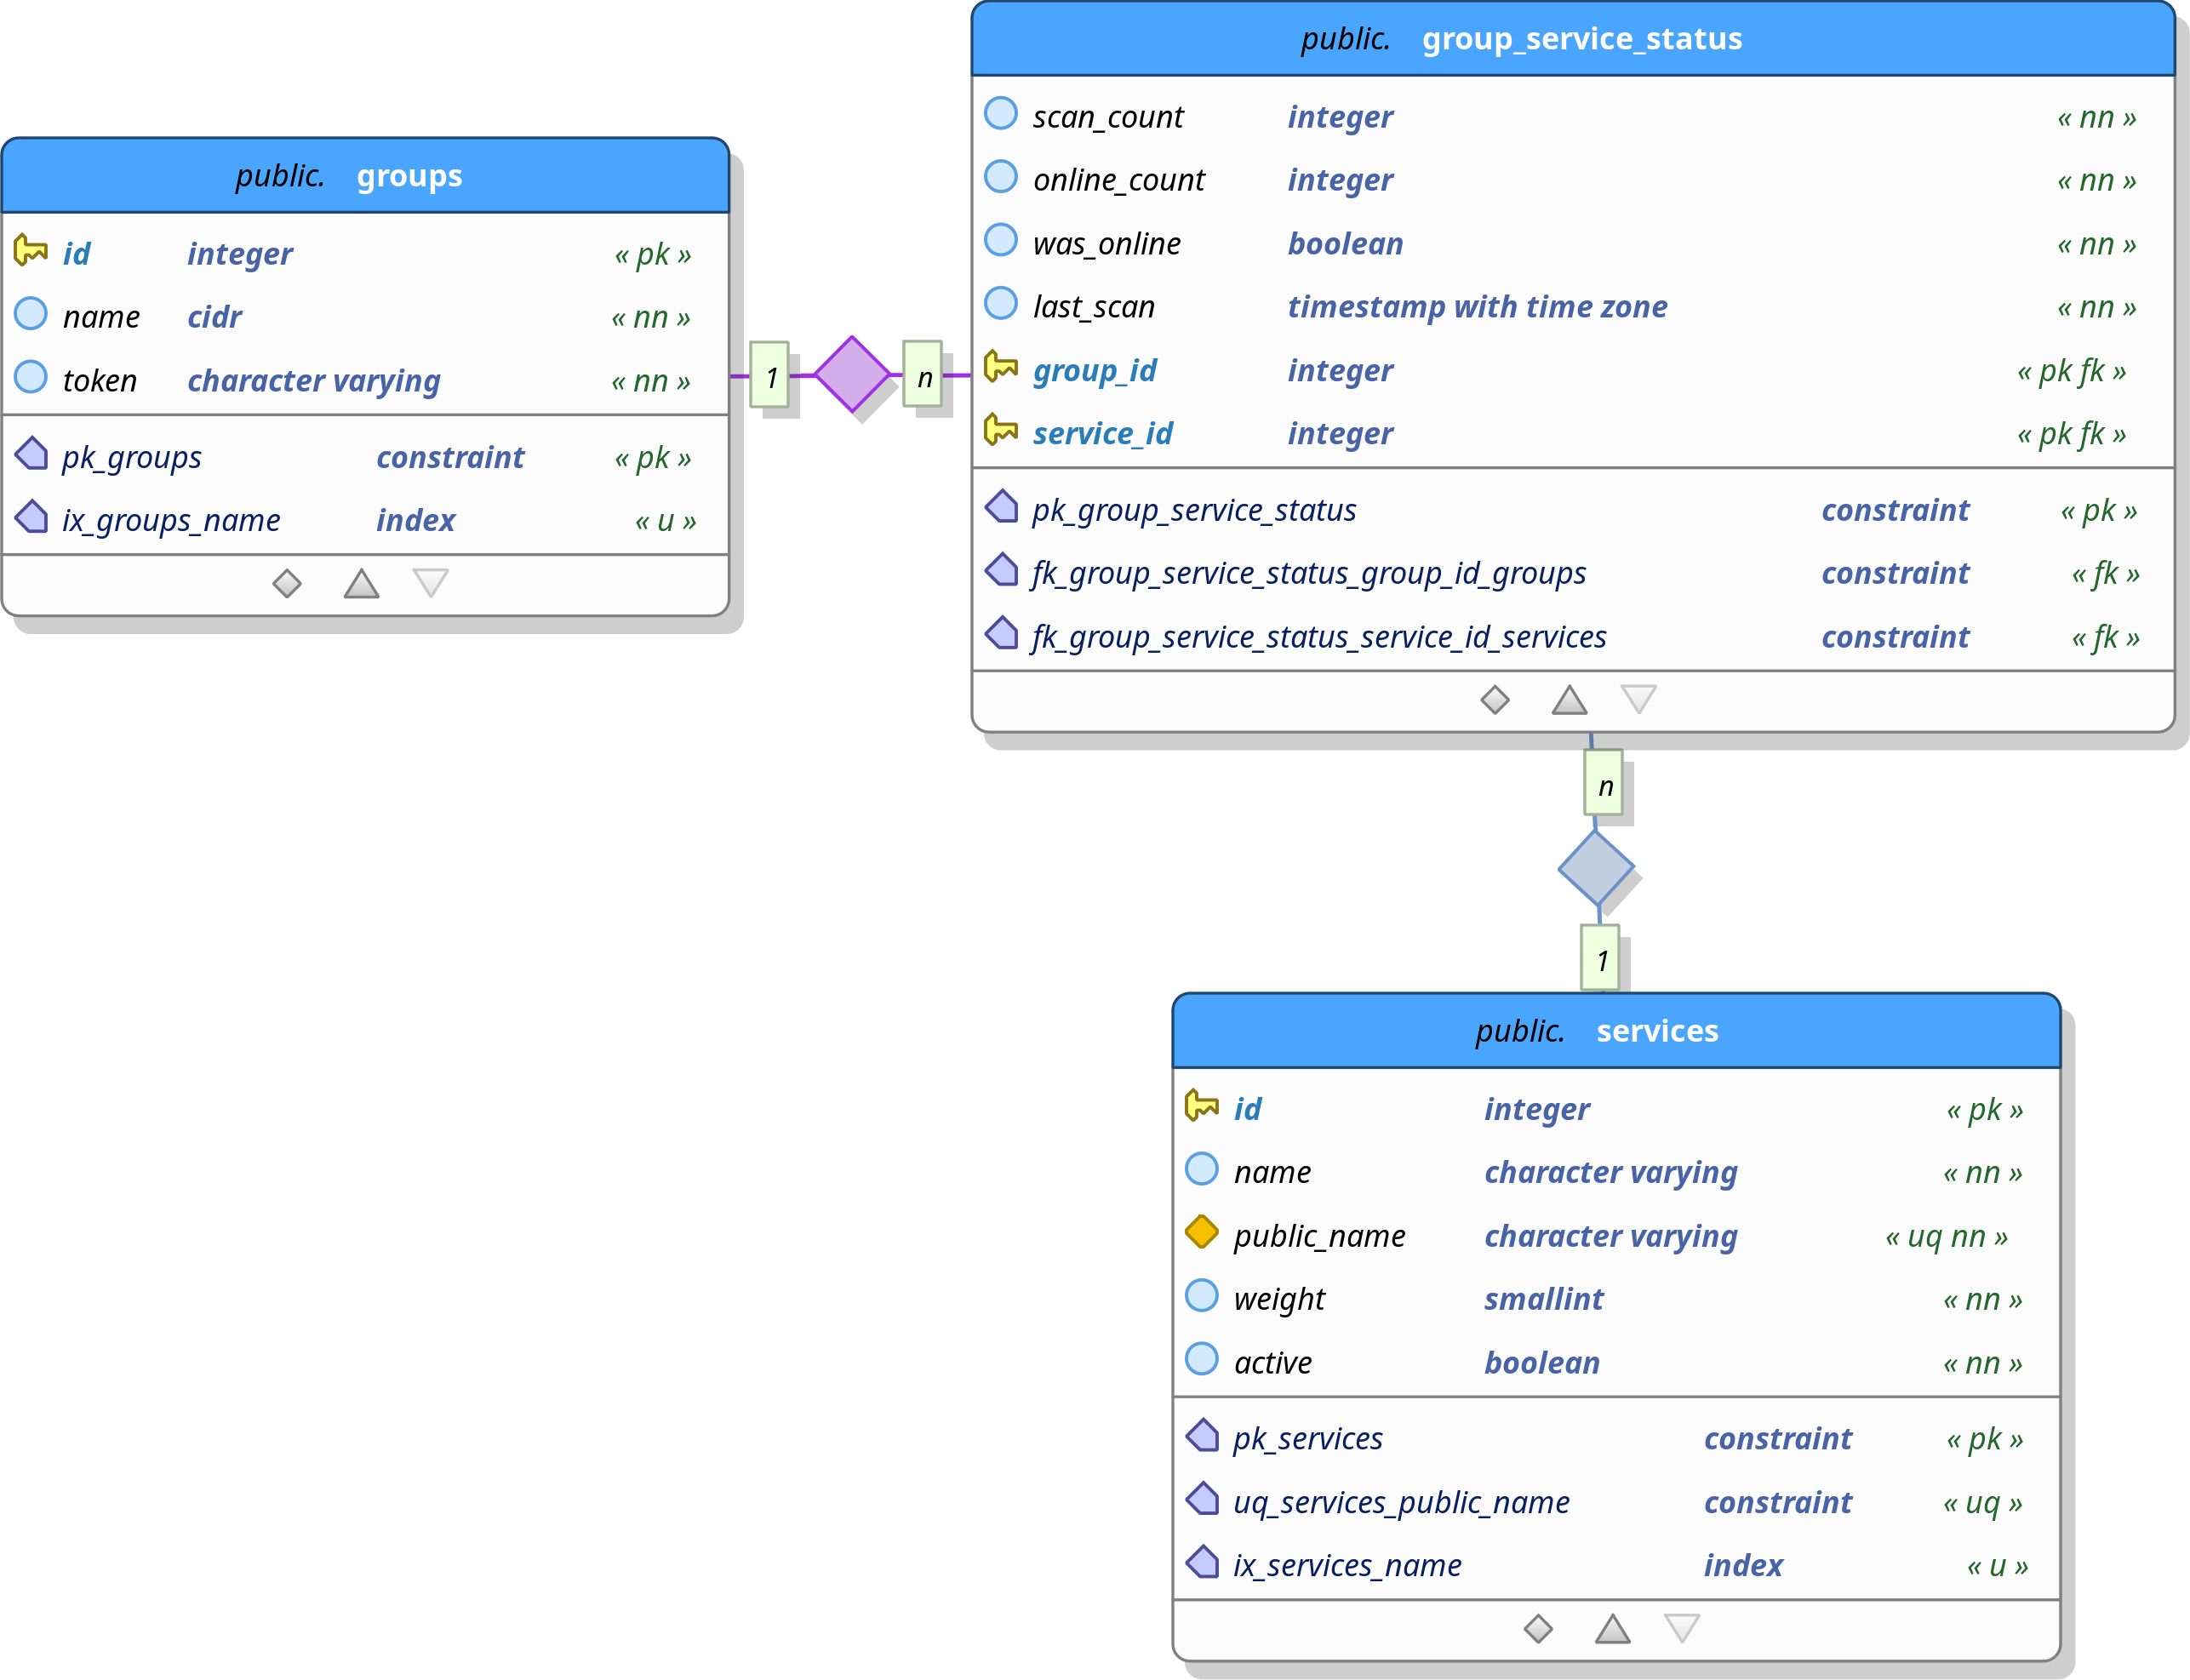
\includegraphics[width=150mm, keepaspectratio]{entwurf/datenbank/service-tabellen}
	\captionof{figure}{Ansicht der Service-Tabellen (ER-Diagramm)}
	\label{fig:db-service-table}
\end{center}

In der \autoref{fig:db-service-table} ist die \textbf{\textit{services}}-Tabelle sowie die n:m-Beziehung zwischen \textbf{\textit{groups}} und \textbf{\textit{services}} zu sehen. Diese wird als Referenztabelle (\textbf{\textit{group\_service\_status}}) mit zwei 1:n-Beziehungen dargestellt.

\subsubsection{Services}
In der \textbf{\textit{services}}-Tabelle sind alle vom Big Brother überwachten Dienste und Schwachstellen eingetragen. Jeder dieser Einträge besteht aus einer eindeutigen ID, dem internen Namen der Operation (\textit{name}), dem angezeigten Namen (\textit{public\_name}) und der Gewichtung im Gesamtergebnis (\textit{weight}). Die Überprüfung der Schwachstelle kann mithilfe des Bool-Wertes \textit{active} an- oder abgeschaltet werden.

\subsubsection{Servicestatus der Gruppen}
In der Referenztabelle \textbf{\textit{group\_service\_status}} wird das Ergebnis der Überprüfung der Schwachstellen und Dienste jeder Gruppe abgespeichert. Dazu wird für die Kombination aus Gruppe und Service ein Eintrag angelegt und die Anzahl der Scans in \textit{scan\_count} und die Anzahl der erfolgreichen Scans in \textit{online\_count} gespeichert. Des Weiteren wird der Zeitpunkt des letzten Scans in \textit{last\_scan} und der Erfolg des letzten Scans in \textit{was\_online} festgehalten. Erfolgreich bedeutet in diesem Kontext, dass die Studierenden die überwachte Schwachstelle ausgebessert und den überwachten Dienst erreichbar gehalten haben.

\subsection{Flagshop-Tabellen}
\begin{center}
	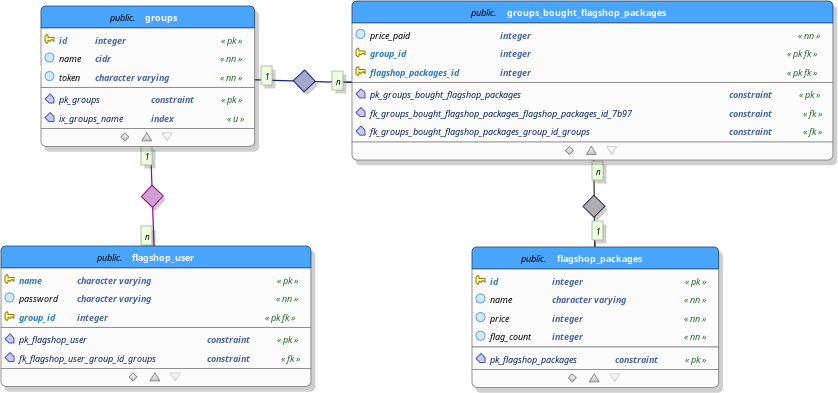
\includegraphics[width=\linewidth, keepaspectratio]{entwurf/datenbank/flagshop-tabellen}
	\captionof{figure}{Ansicht der Flagshop-Tabellen (ER-Diagramm)}
	\label{fig:db-flagshop-table}
\end{center}

Die \autoref{fig:db-flagshop-table} stellt die 1:n-Beziehung zwischen den Tabellen \textbf{\textit{groups}} und \textbf{\textit{flagshop\_user}} dar. Das heißt, dass jeder Gruppe mehrere Flagshop-User zugehörig sein können, jeder User aber genau einer Gruppe angehört. Die n:m-Beziehung zwischen \textbf{\textit{groups}} und \linebreak \textbf{\textit{flagshop\_packages}} wird als Referenztabelle (\textbf{\textit{groups\_bought\_flagshop\_packages}}) mit zwei 1:n-Beziehung dargestellt. Die Referenztabelle beinhaltet die gekauften Flagshop-Pakete pro Team.

\subsubsection{Flagshop-User}
Für die Nutzung des Flagshops müssen die Gruppen einen oder mehrere Flagshop-User anlegen. Diese werden in der Tabelle \textbf{\textit{flagshop\_user}} abgelegt. Hierfür werden neben der erstellenden Gruppe (\textit{group\_id}) auch das Passwort (\textit{password}) und der Name (\textit{name}) abgespeichert. Der Primärschlüssel wird aus der Gruppe und dem Namen gebildet. So ist der Nutzername für die Gruppe eindeutig. Mehrere Gruppen können aber Flagshop-Useraccounts mit demselben Namen anlegen.

\subsubsection{Flagshop-Pakete}
Die betreuenden und administrierenden Personen können Flagshop-Pakete anlegen, die von den Studierenden gekauft werden können. Diese werden in der Tabelle \textbf{\textit{flagshop\_packages}} abgelegt und enthalten Informationen zum Preis (\textit{price}) und der Anzahl der erhaltenen Flags (\textit{flag\_count}). Auch muss ein Name für das Paket über das Feld \textit{name} angegeben werden.

\subsubsection{Gekaufte Flagshop-Pakete}
Die von den Gruppen gekauften Flagshop Pakete werden in der Tabelle \linebreak \textbf{\textit{groups\_bought\_flagshop\_packages}} abgespeichert. Auch wird im Feld \textit{price\_paid} der beim Kauf gezahlte Preis festgehalten, da die Studierenden den Preis eines Flagshop-Paketes beim Kauf reduzieren können. Jedes Paket kann genau einmal von jeder Gruppe gekauft werden, da sich der Primärschlüssel aus Gruppe (\textit{group\_id}) und Paket (\textit{flagshop\_packages\_id}) \linebreak zusammensetzt.

\clearpage
\subsection{Challenge-Tabellen}
\begin{center}
	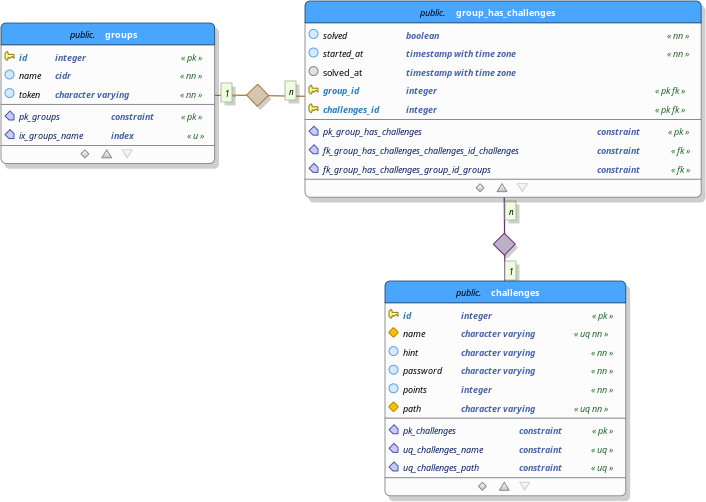
\includegraphics[width=\linewidth, keepaspectratio]{entwurf/datenbank/challenge-tabellen}
	\captionof{figure}{Ansicht der Service-Tabellen (ER-Diagramm)}
	\label{fig:db-challenge-table}
\end{center}
In der \autoref{fig:db-challenge-table} ist die \textbf{\textit{Challenge}} Tabelle und die n:m-Beziehung zwischen den \linebreak Tabellen \textbf{\textit{groups}} und \textbf{\textit{challenges}} zu sehen. Diese Beziehung ist als Verknüpfungstabelle\linebreak (\textbf{\textit{group\_has\_challenges}}) mit zwei 1:n-Beziehung realisiert.

\subsubsection{Challenges}
Die \textbf{\textit{challenges}} Tabelle beinhaltet alle Challenges, die von den Studierenden gelöst werden können. Jede Challenge besitzt eine eindeutige ID. Neben dieser werden für jede Challenge ein Titel in \textit{name}, ein Hinweis in \textit{hint}, das zum Lösen benötigte Passwort in \textit{password}, die Anzahl der Punkte in \textit{points} und der URL-Pfad, über den die Challenge abgerufen werden kann, in \textit{path} gespeichert.

\subsubsection{Gestartete / Abgeschlossene Challenges}
Alle angefangenen und abgeschlossenen Challenges werden in der Tabelle \linebreak
\textbf{\textit{group\_has\_challenges}} abgespeichert. Es werden das Startdatum (\textit{started\_at}) der Challenge, der Status des Abschlusses (\textit{solved}) und bei erfolgreicher Absolvierung der Challenge das Enddatum (\textit{solved\_at}) gespeichert. Durch die Zusammensetzung des Primärschlüssels aus Challenge und Gruppe kann jede Gruppe jede Challenge genau einmal starten und absolvieren.

\subsection{Weitere Tabellen}
\begin{center}
	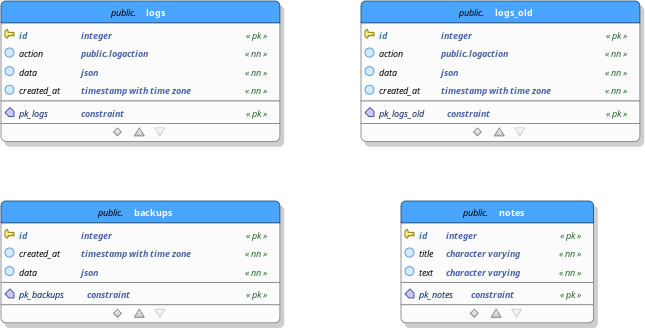
\includegraphics[width=\linewidth, keepaspectratio]{entwurf/datenbank/etc-tabellen}
	\captionof{figure}{Ansicht der weiteren Tabellen (ER-Diagramm)}
	\label{fig:db-etc-table}
\end{center}

Wie in \autoref{fig:db-etc-table} erkennbar, besitzen die Tabellen keine Abhängigkeiten und Verbindungen zu anderen Tabellen. Im Folgenden werden die Tabellen für die Logs, die Notizen und die alten Spielstände vorgestellt.

\subsubsection{Logs}
Um die Aktionen innerhalb der Anwendung nachverfolgen zu können, werden diese in die \textbf{\textit{logs}} Tabelle geschrieben. Jeder Eintrag besteht aus einer ID, einem Enum, in dem der Typ der Aktion festgehalten wird (\textit{action}), einem Zeitpunkt (\textit{timestamp}) und dem Inhalt der Aktion (\textit{data}). 

Innerhalb der \textbf{\textit{logs}} Tabelle werden nur die Aktionen des derzeitig aktiven Spiels gespeichert. Neben diesen werden auch die Aktionen des letzten Spiels in der Tabelle \textbf{\textit{logs\_old}} gespeichert. Sollte ein Spiel beendet werden, werden die Aktionen des alten Spiels mit den neuen Aktionen überschrieben.

\subsubsection{Notizen}
In der Tabelle \textbf{\textit{notes}} soll den betreuenden und administrierenden Personen die Möglichkeit geboten werden, Notizen und Hinweise zum Rahmen und zur Durchführung des Versuches zu platzieren. Diese Notizen können durch die Studierenden eingesehen werden. Dafür werden Titel und Inhalt jeweils in einem String gespeichert. Um einzelne Notizen abrufen zu können, erhalten diese eine eindeutige ID.

\subsubsection{Alte Spiele}
Die Tabelle \textbf{\textit{backups}} soll alle alten Spielstände speichern. Dazu wird jedem Backup eine eindeutige ID zugewiesen und der Zeitpunkt des Erstellens wird in der Spalte \textit{created\_at} abgespeichert. Die Informationen zu einem Spiel sind im JSON-Format in der Spalte \textit{data} abgelegt.